\documentclass[11pt,a4paper]{report}
\usepackage[portuguese]{babel}
\usepackage{listingsutf8}
\usepackage[utf8]{inputenc}
\usepackage[T1]{fontenc}
\usepackage{glossaries}
\usepackage{graphicx}
\usepackage{hyperref}
\usepackage{wrapfig}
\usepackage{float}
\usepackage{natbib}
\usepackage{color}
\usepackage{eurosym}

\newcommand{\HRule}{\rule{\linewidth}{0.5mm}}

\newcommand{\tab}[1]{%
\settowidth{\tabcont}{#1}%
\ifthenelse{\lengthtest{\tabcont < .25\linewidth}}%
{\makebox[.25\linewidth][l]{#1}\ignorespaces}%
{\makebox[.5\linewidth][l]{\color{red} #1}\ignorespaces}%
}%

\begin{document}

%% Página de titulo
\title{\textbf{Jogo de Xadrez implementado em OpenGL} \\ Computação Visual\\Universidade de Aveiro}
\author{Diogo Silva 60337}
\maketitle

\tableofcontents

\definecolor{shadecolor}{RGB}{233,233,233}
\lstset{literate=
		{á}{{\'a}}1 {é}{{\'e}}1 {í}{{\'i}}1 {ó}{{\'o}}1 {ú}{{\'u}}1
		{ã}{{\~a}}1 {ç}{{\c c}}1 {ê}{{\^e}}1 {õ}{{\~o}}1 {€}{{\euro}}1
		{£}{{\pounds}}1,
	basicstyle=\ttfamily\footnotesize,
	numberstyle=\tiny,
	breaklines=true,
	frame=lines,
	tabsize=2,
    showspaces=false,
    showstringspaces=false,
    keywordstyle=\color{blue}\bfseries,
    stringstyle=\color{red},
    commentstyle=\color{blue}\itshape,
    backgroundcolor=\color{shadecolor},
    numbers=left,
    captionpos=t,
    escapeinside={\%*}{*)}
}

\chapter{Introdução}

Este trabalho foi desenvolvido no âmbito da disciplina de Computação Visual do curso de Engenharia de Computadores e Telemática durante o ano curricular 2014/2015, sendo a escolha feita para este projecto foi um jogo de Xadrez (completo, 32 peças) para jogar entre dois jogadores através do mesmo computador, sendo este trabalho uma representação 3D do jogo usando as ferramentas que foram instruídas durante as aulas, neste caso, OpenGL.\\

O desenvolvimento de todo o código ao longo desta aplicação foi feito em C++ usando as bibliotecas de OpenGL, perante isto pode-se encontrar todo o código fonte em: \url{https://github.com/dbtds/chess-opengl}.

O resultado final é descrito ao longo deste relatório, desde detalhes de código (shaders, modelos) até representação gráfica de viewbox, texturas, movimentos, entre outras situações. A imagem seguinte mostra como ficou o trabalho:

\begin{figure}[H]
\centerline{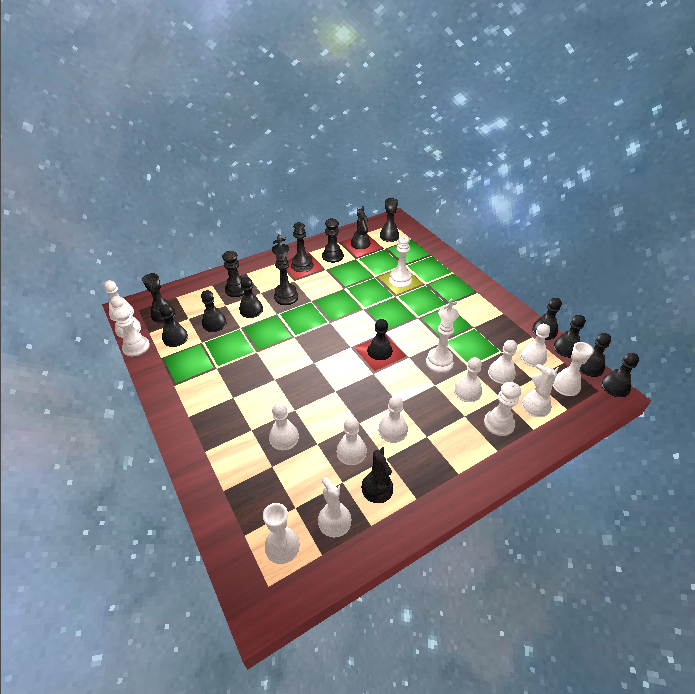
\includegraphics[width=180pt]{images/finalresult.png}}
\caption{Resultado final do Xadrez}
\label{img:complete}
\end{figure}

\chapter{Estrutura da Aplicação}

A aplicação do jogo inicialmente encontrava-se em C, tal como foi sugerido nas aulas, mas devido à necessidade de introduzir o conceito de herança nas peças de Xadrez, passou-se tudo para C++ e realizou-se o desenvolvimento a partir daí.\\

Para compilar o código existe um Makefile disponível no qual foi criado para Linux, apesar de o executável estar disponível de qualquer das formas.

FALTA FALAR DA COMPILAÇÃO MELHOR

\section{Engine do Jogo de Xadrez}

O motor do jogo tem as seguintes funcionalidades como:
\begin{enumerate}
\item{Obter lista das referências para cada peça}
\item{Verificar se o jogo já acabou e quem ganhou}
\item{Verificar de quem é a vez de jogar}
\item{Realizar um movimento}
\item{Mostrar movimentos possíveis de uma peça}
\end{enumerate}

Tal como mostra a figura seguinte, pode-se verificar que estas funcionalidades são acedidas facilmente através da classe Chess.

\begin{figure}[H]
\centerline{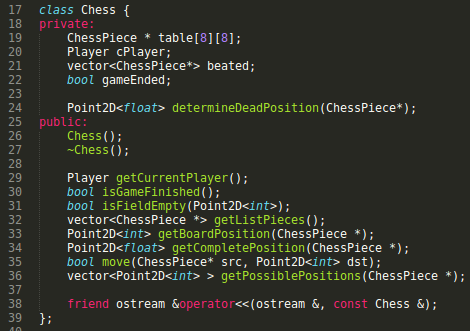
\includegraphics[width=250pt]{images/chess.png}}
\caption{Implementação do Chess}
\label{img:complete}
\end{figure}

Por sua vez, a classe Chess contém uma matrix de 8 por 8 (64 lugares) em que no ínicio, estão 32 ocupadas e as restantes apontar para NULL, esta matrix é uma matrix de referências de Peças de Xadrez, mais precisamento, objectos do tipo ChessPiece (descritos detalhadamente na secção seguinte).

\subsection{Peças do Xadrez}

As peças de Xadrez têm um módulo do qual permite destinguir a qual jogador pertence a peça, o tipo da peça (se é um Rei, um Cavalo, etc..). Consecutivamente, também é o que permite destinguir movimentos das peças.\\

Todas as peças herdam uma classe principal chamada ChessPiece, que contém as funcionalidades referidas anteriomente, tal como mostra a figura seguinte:

\begin{figure}[H]
\centerline{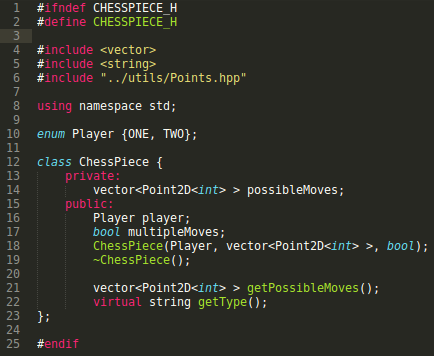
\includegraphics[width=250pt]{images/chesspiece.png}}
\caption{Implementação do ChessPiece}
\label{img:complete}
\end{figure}

Tal como foi referido, todas as peças têm de indicar na sua inicialização a lista de movimentos possíveis, se são movimentos multíplos ou não e o jogador a qual pertence, na figura seguinte pode-se ver o exemplo da implementação da Rainha, em que mostra que os movimentos possíveis são em todas as casas as sua volta e são movimentos multíplos.

\begin{figure}[H]
\centerline{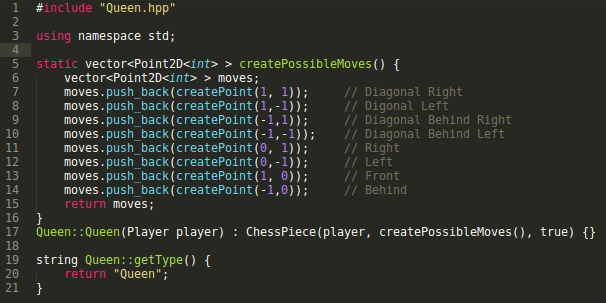
\includegraphics[width=380pt]{images/queen.png}}
\caption{Implementação da Peça Rainha}
\label{img:complete}
\end{figure}

\section{Desenvolvimento OpenGL}

Relativamente a implementação da parte gráfica da aplicação, decidiu-se dar continuação a estrutura já existentes das aulas, tendo os seguintes ficheiros:
\begin{enumerate}
\item{init.cpp, que inicia todos os modelos, fontes de luz, estruturas, janela e callbacks}
\item{models.cpp, que permite ler os ficheiros obj do formato oficial}
\item{globals.cpp, contém algumas variaveis globais para permitir fácil manipulação durante o uso de callbacks}
\item{callbacks.cpp, este ficheiro é o que trata de reescrever a imagem, trata também ainda dos movimentos do rato e cliques do teclado}
\item{shaders.cpp, este ficheiro é o que carrega o vertex e o fragment shader}
\end{enumerate}

Para além deste ainda foram criados dois ficheiros, um LightModel.cpp que contém apenas todas as caracteristicas necessárias para a representação de um foco de iluminação, tais como, posição do foco, intensidade do foco e intensidade da luz ambiente.
O outro ficheiro, é o ficheiro GraphicModelChess.cpp que contém as caracteristicas gráficas de cada modelo de Xadrez (este ficheiro é descrito detalhamente na secção seguinte).

\subsection{Modelos}

\subsubsection{Estrutura do GraphicModelChess}

A classe GraphicModelChess contém todas as caracteristicas gráficas de cada modelo:
\begin{enumerate}
\item{Número de vertíces}
\item{Lista de vertíces}
\item{Lista das normais}
\item{Valores de deslocamento, rotação e de redimensionamento}
\item{Coeficiente Ambiente, Difusão, Especular e Phong}
\end{enumerate}

Para além deste valores, ainda contém uma referência para o respectivo modelo de Xadrez, ou seja, objecto ChessPiece.

A figura seguinte mostra o cabeçalho deste ficheiro:

\begin{figure}[H]
\centerline{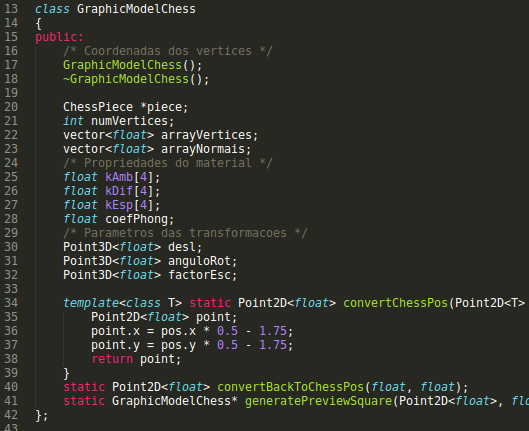
\includegraphics[width=300pt]{images/graphicmodelchess.png}}
\caption{Cabeçalho do GraphicModelChess}
\label{img:complete}
\end{figure}

Ainda se pode verificar a existência de 3 funções estáticas, duas das quais servem para converter coordenadas do tabuleiro de Xadrez para coordenadas do mundo 3D, e vice-versa. A outra função serve para gerar modelos quadrados que vão servir para representar todas as alternativas possíveis de cada movimento.

\subsubsection{Load de cada modelo de Xadrez}

As peças do Xadrez foram retiradas de modelos já existentes num projecto Open Source \url{https://code.google.com/p/pwag-chessboard/}, desse projecto foram retirados do directório /trunk/Chess/Chess/Models.\\

Sendo que esses modelos foram todos optimizados usando o programa Blender de maneira a ficarem da forma pretendida, tal como, colocar a base no plano xOy, ou seja, z = 0.

Após a recolocação dos modelos, foram todos exportados para ficheiros .obj no formato oficial.

Apesar de fazer a leitura do modelo oficial dos ficheiros obj, apenas são carregados os vertices, as normais e as faces, deixando de foram os vertices das texturas.

O load genérico dos ficheiros obj encontra-se em /src/models.cpp.

\subsection{Shaders}

Inicialmente os shaders apenas estavam a ser usados para a representação das cores, não fazendo qualquer procesamento na gráfica, mas houve a necessidade de implementar a iluminação nos shaders devido ao tentar fazer uma animação mais complexa e notar-se que a imagem não era completamente fluída porque o tempo que o CPU demorava a fazer os calculos das iluminações de cada vertice era superior ao tempo da rotação, verificando-se um delay no movimento.\\

Sendo assim, havia duas opções, tornar a animação mais rudimentar, ou passar a iluminação para os shaders (fazendo com que a gráfica processa-se a animação).

\begin{figure}[H]
\centerline{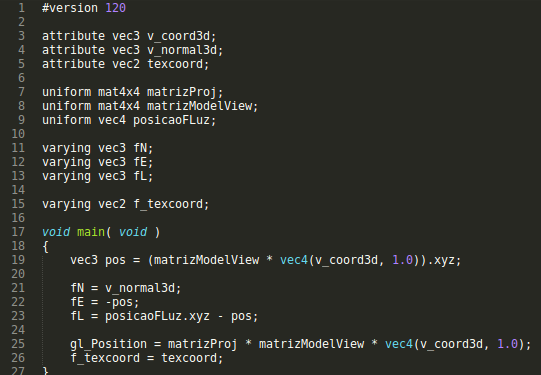
\includegraphics[width=300pt]{images/vertexshader.png}}
\caption{Vertex Shader}
\label{img:complete}
\end{figure}

Como se pode verificar no vertex shader é feito os calculos do ponto relativamente a um vertice, a sua posição, consoante a matrix projecção e o modelo, para além disso, ainda é calculado alguma fracções que vão ser usadas mais tarde pelo fragment shader, estas precisam de ser calculadas no vertex porque a iluminação depende da posição do vertice e do foco de iluminação.\\

Ainda se pode verificar que as coordenadas das texturas são passadas para o fragment shader.

\begin{figure}[H]
\centerline{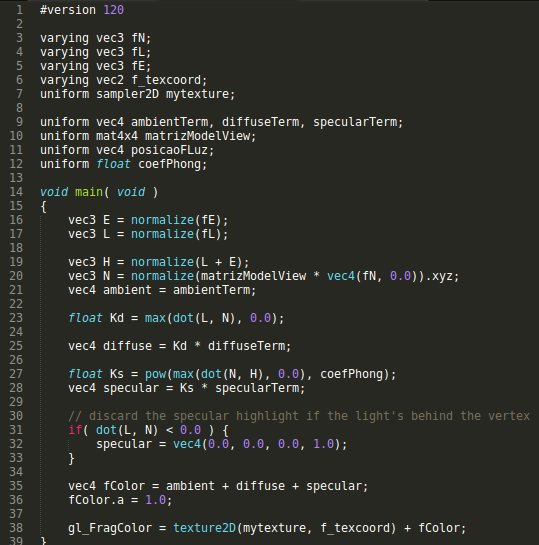
\includegraphics[width=300pt]{images/fragmentshader.png}}
\caption{Fragment Shader}
\label{img:complete}
\end{figure}

No fragment shader pode-se verificar que são usadas as variaveis passadas pelo Vertex Shader, neste caso, fE, fN e fL, calculando a respectiva cor do vertice, dando o efeito de iluminação pretendido.\\

Para realizar esta parte do código foi utilizado os slides dados na teórica das aulas de Computação Visual no ficheiro PDF ``Métodos de Iluminação e Sombreamento (PDF)'' disponível em \url{http://sweet.ua.pt/jmadeira/CV/CV_07_Ilumina%C3%A7%C3%A3o_e_Shading_BSS_JM.pdf} nos slides 50 a 53.\\

Ainda se pode verificar que as texturas são introduzidas com o texture2D que permite aplicar uma cor RGB a uma coordenada específica, fazendo isto com todas as coordendas, para além disto, ainda se pode verificar que dá-se igual importância a textura e a iluminação, apesar de não ser o melhor método funciona relativamente bem.

\chapter{Aspectos Importantes do Trabalho}

\section{Interacção com o utilizador}

\subsection{Clique nas peças do Xadrez (Interacção Directa)}

\subsection{Manipulação do cenário}

\section{Iluminação na Placa Gráfica}

\section{Texturas}

\section{Skybox}

\section{Representação Gráfica}

\subsection{Peças de Xadrez}

\subsection{Movimentos possíveis}

\subsubsection{Distinção de movimentos}

\subsection{Peças mortas}

\chapter{Conclusão}
%



%% Glossário (Lista de acronimos)
%\printglossaries
%\addcontentsline{toc}{chapter}{Glossário}

%% Bibliografia
%\bibliographystyle{plain}
%\bibliography{report}
%\addcontentsline{toc}{chapter}{Bibliografia}

%% Lista de Figuras
\listoffigures
%\addcontentsline{toc}{chapter}{Lista de figuras}
%% Lista de Tabelas
% Não foi incluido list of tables porque não foi preciso utilizar nenhuma tabela neste trabalho.

%\listoftables
%\addcontentsline{toc}{chapter}{Lista de tabelas}

\end{document}